\chapter{Introdução}
\label{cap:introducao}

A fala é a forma mais natural de comunicação que uma pessoa tem no cotidiano.
Bem recentemente nossos computadores têm se tornado cada vez melhores na complexa tarefa que é interagir conosco usando a fala. 
Não é claro quando os humanos começaram a falar propriamente uns com os outros mas através do nosso longo período de evolução fomos adquirindo maneiras mais precisas, específicas e claras de expressar e comunicar ideias e transmitir informações através de som com o uso de uma linguagem.

O processo todo de interação engloba uma sequência de atividades (Fig. \ref{fig:processo_de_fala}): a organização de uma ideia em palavras, a expressão dessas palavras por um meio vocal, a transmissão desse meio até o aparelho auditivo do par que se interage, a conversão das onda sonora pelo aparelho auditivo do ouvinte para sinais elétricos transmitidos e processados pelo cérebro, o processamento desses sinais em uma linguagem e finalmente a interpretação desses sinais em um significado completo.

\begin{figure}
	\centering
	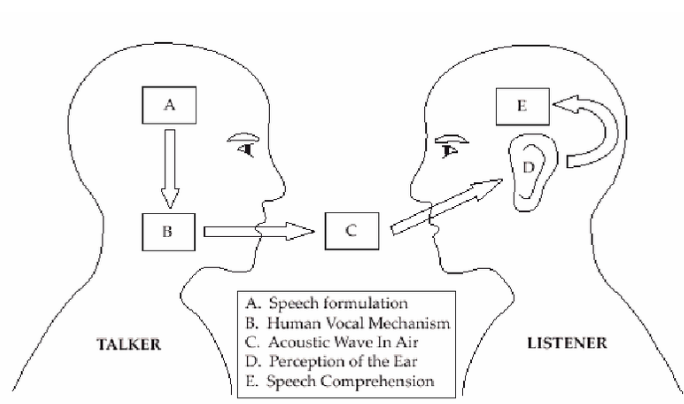
\includegraphics[width=\textwidth]{figuras/processo_de_fala.png}
	\caption[Diagrama do Processo de Produção/Percepção da Fala]{Diagrama do Processo de Produção/Percepção da Fala \cite{speech_process}}
	\label{fig:processo_de_fala}
\end{figure}

Sistemas de STT (\textit{Speech to Text}) foca no processo D representado no diagrama, onde o interesse é apenas a compreensão da mensagem transmitida. O processo C de transmissão no meio é interpretado através de um processo de quantização e amostragem do contínuo de modo a ser possível seu processamento por computadores. O papel de formulação e compreensão da mensagem transmitida representado no diagrama pelas letras A e E, respectivamente, já teve vários candidatos ao longo dos anos, desde sistemas especialistas, diálogos com chatbots até complexas redes neurais para respostas de questões genéricas \cite{question_1:DBLP:journals/corr/abs-1805-08092, question_2:DBLP:journals/corr/abs-1806-08730, pointer_1:DBLP:journals/corr/XiongZS16, pointer_2:DBLP:journals/corr/abs-1801-08290, pointer_3:DBLP:journals/corr/abs-1801-09251, pointer_4:DBLP:journals/corr/WangJ16a}. O intuito desse trabalho é o estudo da replicação do modelo de fala, representado pela letra B, e pela síntese e transmissão do mesmo por um meio, a letra C. Não é intuito desse trabalho dar ênfase a nenhum dos outros momentos de produção, percepção e interação através da fala mas dada uma intercessão natural existente entre as atividades de comunicação alguns cuidados e algumas técnicas são compartilhadas entre processos.

As primeiras tentativas documentadas de estratégias para síntese de fala datam do século XVIII \cite{vonKempelen1791}. As mais diversas técnicas foram tomando forma e evoluindo com o tempo de modo que, comparativamente, algumas são mais simples, outras mais portáteis, outras mais genéricas, todas visando algum aspecto distinto cujo algum outro modelo era ineficiente para a aplicação desejada. Abordo com ênfase nesse trabalho a síntese de fala neural que é uma das estratégias mais genéricas dentre as disponíveis atualmente pois permite capturar as características necessárias para a síntese nas mais diversas fontes e dos mais diversos falantes.

\section{Organização do Trabalho}
\label{sec:organizacao_trabalho}

%Contextualização Histórica e Introdução Teórica dos blocos de redes neurais
Começamos esse trabalhos contextualizando técnicas implementadas anteriormente e técnicas usadas amplamente ainda hoje, caracterizando assim um breve revisão histórica das abordagens para síntese de fala. Após contextualizar os modelos legados iremos apontar os atuais estados da arte para síntese de fala neural focando na sua construção modular e discutir seus aspectos positivos e negativos comparativamente. Após introduzir os modelos neurais estudados desejamos dar ao leitor uma introdução dos conceitos utilizados em cada modelo. 

%Análise Comparativa das Línguas, Análise dos Dados Divulgados, Análise dos Dados propostos
Selecionamos então um modelo neural para discorrer com maiores detalhes e buscamos estudar seu comportamento com a língua portuguesa. Iniciamos a discussão através da análise dos dados e de um possível enviesamento de performance do modelos tendo em vista a majoritariedade das análise focando apenas a síntese no inglês. Levantamos um estudo observando diferenças entre português e inglês como diversidade e frequência de fonemas, sotaques, dimensão de palavras existentes, dimensão de palavras usadas cotidianamente. Tendo essa análise comparativa entre os dados de treinamento esperamos ter mais facilidade em criticar o comportamento do modelo tanto no inglês quanto no português.

%Construção dos dados de treino em Português
Apontamos uma estratégia genérica para construção de um conjunto de dados com frases/palavras curtas em português através da extração de áudios de vídeos legendados. Usamos nesse trabalho áudios de vídeos do YouTube baseado nas segmentações automáticas das legendas. Apontamos as vantagens e desvantagens desse método e como parâmetro comparativo elegemos uma situação de ilusão auditiva \cite{auditory_illusion} para observar se o modelo é capaz de produzir alguma síntese similar. 
%QUESTION: Discutir em trabalhos futuros outras possíveis técnicas para construção de conjuntos de dados? Uma possível segmentação de palavras por silêncio é possível. Um modelo similar ao Listen Attention Watch também é possível de ser treinado APENAS para produzir um conjunto de dados. Mas a utilização de outro modelo traria uma possível inconsistência transferida que fica completamente invisível no treinamento.

%Parâmetros de treino, frameworks utilizados, métricas usadas para avaliação
Discutimos então os detalhes técnicos de implementação, disponibilizamos os parâmetros utilizados no treinamento, discutimos as métricas usadas para avaliação da performance do modelo durante o treino e então sintetizamos algumas frases referenciais para poder avaliar a performance do sistema na avaliação humana. Essas frases selecionadas sintetizadas são avaliadas por um grupo de ouvintes que dão notas cujos valores mais altos correspondem aos trechos mais realistas.
%QUESTION: No caso é necessário obter trechos de áudio que sejam autorizados por seus falantes para síntese? Eu precisaria, por exemplo, entrar em contato com os donos dos vídeos selecionados para solicitar autorização expressa ou apenas por estar disponibilizado na internet já seria suficiente? Ou ainda isso seria variável de acordo com a disponibilidade de compartilhamento do vídeo?
\section{Contribuições}
\label{sec:contribucoes}
Buscamos nesse trabalho:
\begin{enumerate}
    \item Propor uma estratégia de construção escalável e automática de uma base de dados não-estruturados disponíveis em alta escala para qualquer língua
    %QUESTION: Vale a pena criticar esse ponto tendo em vista os problemas mais genéricos de NLP?
    \item Avaliar a performance do estado da arte de síntese de fala com estratégias usando redes neurais na língua portuguesa comparativamente ao inglês
    %QUESTION: Vale a pena criticar o modelo tendo em vista questões técnicas de RNN, por exemplo?
    \item Levantar aspectos interpretáveis do aprendizado do modelo neural de modo a facilitar pos\-síveis otimizações futuras %Usar a construção modular como argumento
    %QUESTION: Vale a pena criticar um modelo ininterpretável que tenha uma performance e generalização melhor junto à perda total da compreensão?
    \item Propor um modelo de \emph{embeddings} que faça jus à similaridade fonética das palavras de modo que na conversão grafema $\rightarrow$ fonema possamos ter uma contextualização mais próxima à falada possível
    %QUESTION: Vale a pena propor o modelo e disponibilizá-lo baseado em um dicionário fonético ou focar na sua interpretabilidade? Talvez um modelo alinhado a uma base maior como a wikipédia seja uma boa base para frequência de palavras de modo a produzir um sistema fonético mais alinhado a frequência
\end{enumerate}

\newpage